% !!Não alterar!!! Este comando inclui as configurações da classe do documento
\documentclass[
  12pt,
  a4paper,
]{template/td}

%%%%%%%%%%%%%%%%%%%%%%%%%%%%%%%%%%%%%%%%%%%%%%%%%%%%%%%
%  Preencha os dados para títutlo e capa da publicação%
%%%%%%%%%%%%%%%%%%%%%%%%%%%%%%%%%%%%%%%%%%%%%%%%%%%%%%%

\tdtitle{TÍTULO} % Título do Texto para Discussão

\tdautor{Autor 1}{Afiliação 1} % Autor 1 e afiliação

\tdautor{Autor 2}{Afiliação 2} % Autor 2 e afiliação ....
%% Se for necessário adcionar mais autores, repita com comando \tdautor{autor}{afiliação}

\tdjel{XXX; XXX; XXX.} %% JEL code

\tdpchave{xxxxx; xxxx; xxxx; xxxx.} % palavras-chave

\tdkwords{xxxxx; xxxx; xxxx; xxxx.} % keywords

\tdnum{xx} % número do TD

\tdcidade{xxxx} % cidade

\tdano{xxxx} % ano

\tdedicao{xª} % edição

\tddoi{xx.xxx/xxxxxxx} % DOI

\tdissn{xxxx-xxxx} % ISSN

%%%%%%%%%%%%%%%%%%%%%%%%%%%%%%%%%%%%%%%%%%%%%%%%%%%%%%%
%%%%%%%%%%%%%%%%%%%%%%%%%%%%%%%%%%%%%%%%%%%%%%%%%%%%%%%

% Adcione o arquivo com as refrêncas bilbigráficas (default: rerefrencia.bib)
\addbibresource{referencia.bib}

% !!Não alterar!!! Este comando inclui configurações padrao da publicação no preamble do documento tex
% metadados do PDF
\makeatletter
\hypersetup{
  pdftitle={\@tdtitle},
  pdfauthor={Autor 1; Autor 2},
  pdflang={pt},
  pdfkeywords={\@tdkwords},
  hidelinks}
\makeatother

% maketitle
\makeatletter
\title{\large\bfseries \@tdtitle}
\makeatother
\author{}
\date{}

\begin{document}

% !!Não alterar!!! Este comando inclui as configurações da capa da publicação
% frontpage e expediente
\ThisCenterWallPaper{1}{images/td_capa_v2.png}
\clearpage
\thispagestyle{empty} 
\newgeometry{top=90mm, left=10mm, right=20mm}
\makeatletter
\begin{tikzpicture}[remember picture, overlay]
   \node [anchor=north east, inner sep=105pt] at ([xshift=2.5cm]current page.north east) {
      \begin{minipage}{.3\textwidth}
         \fontsize{70}{78}\selectfont
         \color{white}
         \arialboldfont{\@tdnum}
      \end{minipage}
   };
\end{tikzpicture}
\makeatother
\makeatletter
\fboxsep=15pt\fbox{\begin{minipage}[c]{1\textwidth} 
{\centering
{\large\bfseries \@tdtitle \par}
}
\vspace{1.5cm} 
{\footnotesize \textbf{Autores(as):}} \par
\gerautorlist
\vspace{1cm}
{\footnotesize \textbf{Cidade:} \hspace{3.10cm} \@tdcidade} \newline
{\footnotesize \textbf{Editora:} \hspace{3cm} Instituto de Pesquisa
Econômica Aplicada -- Ipea} \newline
{\footnotesize \textbf{Ano:} \hspace{3.55cm} \@tdano} \newline
{\footnotesize \textbf{Edição:} \hspace{3.10cm} \@tdedicao} \newline
{\footnotesize \textbf{JEL:} \hspace{3.60cm} \@tdjel} \newline
{\footnotesize \textbf{DOI:}\hspace{3.65cm} \@tddoi} \newline
\end{minipage}}
\makeatother
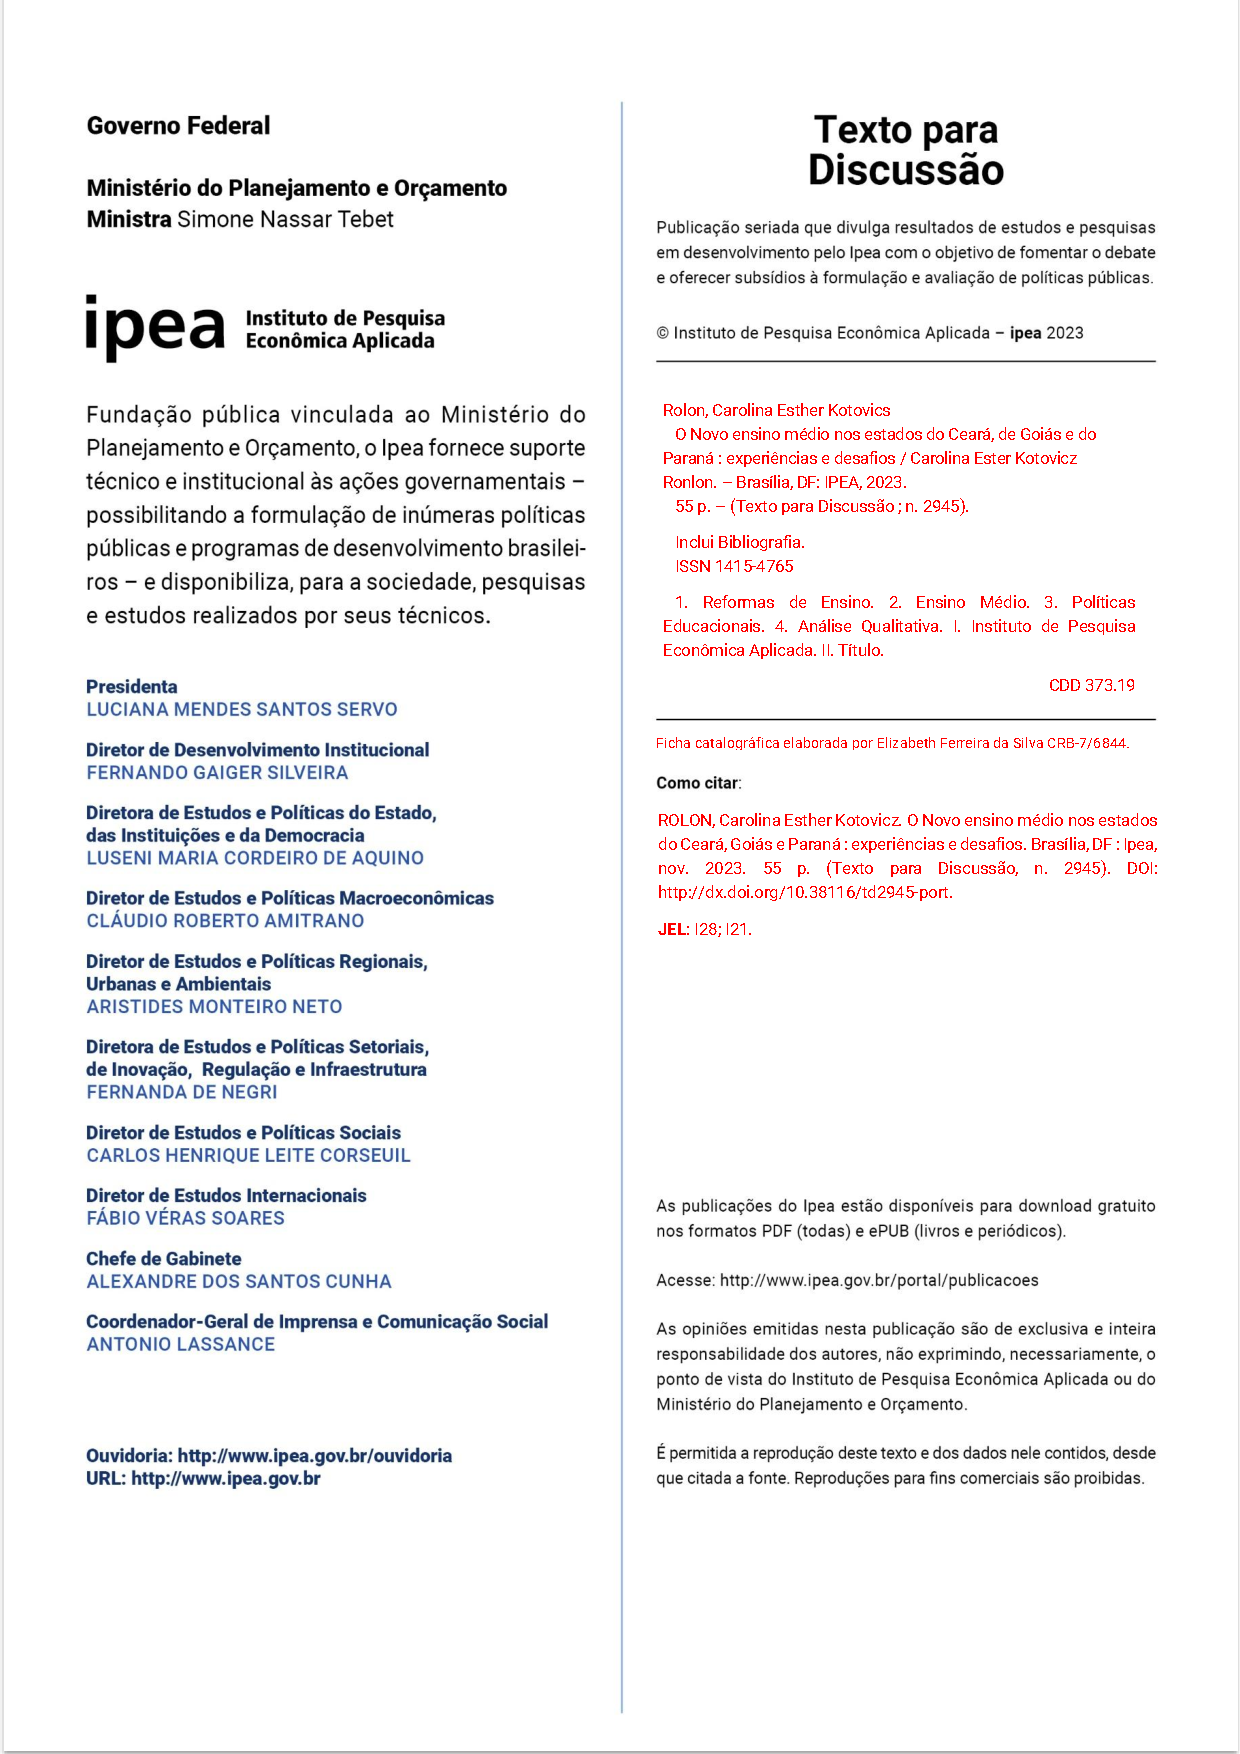
\includepdf[pages={1}, scale=1]{td_expediente_ficha.pdf}
\clearpage 
\pagenumbering{arabic}
\setcounter{page}{1}
\restoregeometry

\maketitle

% !!Não alterar!!! Estes comandos configuram aspectos visuais da padrão da publicação
\thispagestyle{fancy}
\setstretch{1.24}

% Sinopse
\section*{SINOPSE\footnote{Nota de rodapé}}

Lorem ipsum dolor sit amet, consectetur adipiscing elit. Etiam dapibus
fringilla erat, a pulvinar mi. Duis consequat maximus magna, ut rutrum
ipsum efficitur nec. Duis vel erat sollicitudin, aliquet quam a, sodales
mi. Ut eu viverra diam. Pellentesque blandit lorem iaculis, pretium
neque et, ultrices libero. Maecenas fermentum, leo sit amet pharetra
posuere, nulla augue mattis felis, nec vestibulum tellus dolor efficitur
mauris. Ut a tellus vitae quam efficitur dictum suscipit pulvinar felis.
Interdum et malesuada fames ac ante ipsum primis in faucibus. Nunc
tempus dolor a urna scelerisque suscipit.

% !!Não alterar!!! Os comandos abaixo preenchem palavra-chave e JEL automaticamente
\makeatletter
\textbf{Palavras-chave:} \@tdpchave
\makeatother

\makeatletter
\textbf{JEL:} \@tdjel
\makeatother

% Sinopse
\section*{ABSTRACT}

Lorem ipsum dolor sit amet, consectetur adipiscing elit. Etiam dapibus
fringilla erat, a pulvinar mi. Duis consequat maximus magna, ut rutrum
ipsum efficitur nec. Duis vel erat sollicitudin, aliquet quam a, sodales
mi. Ut eu viverra diam. Pellentesque blandit lorem iaculis, pretium
neque et, ultrices libero. Maecenas fermentum, leo sit amet pharetra
posuere, nulla augue mattis felis, nec vestibulum tellus dolor efficitur
mauris. Ut a tellus vitae quam efficitur dictum suscipit pulvinar felis.
Interdum et malesuada fames ac ante ipsum primis in faucibus. Nunc
tempus dolor a urna scelerisque suscipit.

% !!Não alterar!!! Os comandos abaixo preenchem keywords e JEL automaticamente
\makeatletter
\textbf{Keywords:} \@tdkwords
\makeatother

\makeatletter
\textbf{JEL:} \@tdjel
\makeatother

\newpage{}

% Primeira seção
\section{SEÇÃO}

Lorem ipsum dolor sit amet, consectetur adipiscing elit. Etiam dapibus
fringilla erat, a pulvinar mi. Duis consequat maximus magna, ut rutrum
ipsum efficitur nec. Duis vel erat sollicitudin, aliquet quam a, sodales
mi. Ut eu viverra diam. Pellentesque blandit lorem iaculis, pretium
neque et, ultrices libero. Maecenas fermentum, leo sit amet pharetra
posuere, nulla augue mattis felis, nec vestibulum tellus dolor efficitur
mauris. Ut a tellus vitae quam efficitur dictum suscipit pulvinar felis.
Interdum et malesuada fames ac ante ipsum primis in faucibus. Nunc
tempus dolor a urna scelerisque suscipit.

\citep{nome2023} % referência entre parênteses
\citet{nome2023} % refrência no texto, sem parêntese

% Subseção
\subsection{Subseção}

Lorem ipsum dolor sit amet, consectetur adipiscing elit. Etiam dapibus
fringilla erat, a pulvinar mi. Duis consequat maximus magna, ut rutrum
ipsum efficitur nec. Duis vel erat sollicitudin, aliquet quam a, sodales
mi. Ut eu viverra diam. Pellentesque blandit lorem iaculis, pretium
neque et, ultrices libero. Maecenas fermentum, leo sit amet pharetra
posuere, nulla augue mattis felis, nec vestibulum tellus dolor efficitur
mauris. Ut a tellus vitae quam efficitur dictum suscipit pulvinar felis.
Interdum et malesuada fames ac ante ipsum primis in faucibus. Nunc
tempus dolor a urna scelerisque suscipit. 
\begin{table}[!h]

% Modelo de tabela
\caption{\textbf{Título da tabela}}
\fontsize{11}{13}\selectfont
\begin{tabular}[t]{>{\raggedright\arraybackslash}m{3.5cm}|>{\raggedright\arraybackslash}m{3.5cm}|>{\raggedright\arraybackslash}m{3.5cm}|>{\raggedright\arraybackslash}m{3.5cm}}
\hline
Tipo de dado & Descrição & Fonte & Ano\\
\hline
Estabelecimentos de saúde & Localização dos estabelecimentos de saúde vinculados ao SUS segundo nível de complexidade: atenção básica e alta complexidade & CNES, Ministério da Saúde & 2019\\
\hline
Dados sociodemográficos & Quantidade de pessoas segundo sexo, idade e cor/raça; média da renda domiciliar per capita & Censo Demográfico, IBGE & 2010\\
\hline
Malha viária & Dados espaciais das vias, incluindo trechos para pedestres & OpenStreetMap (OSM) & nov/20\\
\hline
Topografia & Modelo digital de elevação, com resolução espacial de aproximadamente 30 metros & Shuttle Radar Topography Mission (SRTM) – Nasa & 2000\\
\hline
Transporte Público & Dados de transporte público em formato GTFS & Agências de transporte & 2019\\
\hline
Histórico de velocidade de automóveis & Dados da malha viária com atributos de tráfego e sentido da via para automóveis & Streetmap Premium (ESRI/Here) & 1o trimestre de 2018 ao 1o trimestre de 2020\\
\hline
\multicolumn{4}{l}{\rule{0pt}{1em}\footnotesize{Nota de rodapé.}}\\
\end{tabular}
\end{table}

% Comando para incluir figuras
\figuratd{images/imagem.png}{Título da figura}{Nota de rodapé.}{fig-rotulo}

% Incluir referências bibliográficas
\printbibliography

\end{document}